\pagebreak
\section{Timer}
Parte fondamentale per il funzionamento del microcontrollore è il Timer. In particolare, il timer è fondamentale per scandire il rateo delle operazioni della CPU e per dare un tempo di esecuzione alle periferiche.\\

Nel microcontrollore che abbiamo usato non c'è un singolo timer e ognuno ha caratteristiche, precisione e funzionalità diverse. 
Per i nostri scopi, noi abbiamo interagito con il Timer 6.

\subsection{Funzionamento}

\begin{figure}[h]
    \centering
    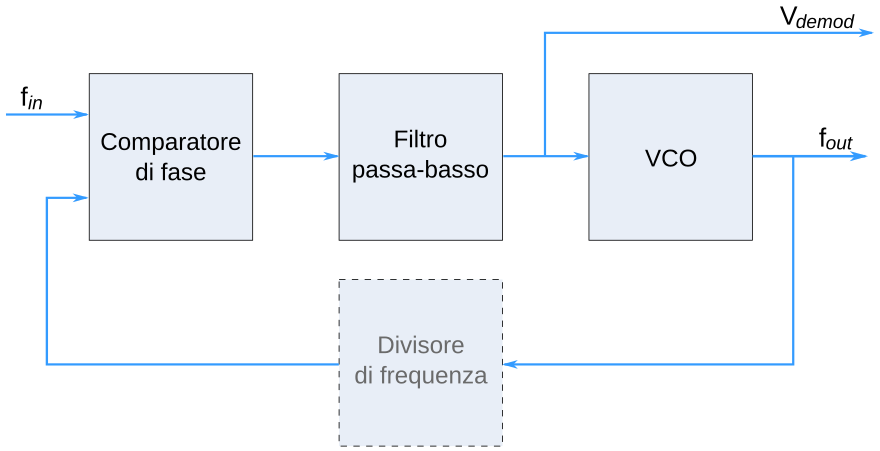
\includegraphics[width=0.7\linewidth]{microcontrollore/assets/PLL1_it.png}
    \caption{Schema di funzionamento del Timer}
    \label{fig:Timer}
\end{figure}